\documentclass[12pt]{article}
\usepackage[utf8]{inputenc}
\usepackage{float}
\usepackage{amsmath}
\usepackage{amssymb}

\usepackage{tikz}
\usetikzlibrary{positioning}

\usepackage[hmargin=3cm,vmargin=6.0cm]{geometry}
%\topmargin=0cm
\topmargin=-2cm
\addtolength{\textheight}{6.5cm}
\addtolength{\textwidth}{2.0cm}
%\setlength{\leftmargin}{-5cm}
\setlength{\oddsidemargin}{0.0cm}
\setlength{\evensidemargin}{0.0cm}

%misc libraries goes here
\usepackage{fitch}

\begin{document}

\section*{Student Information } 
%Write your full name and id number between the colon and newline
%Put one empty space character after colon and before newline
Full Name :  Alperen OVAK\\
Id Number :  2580801\\

% Write your answers below the section tags
\section*{Answer 1}

The \( Q_n \) cube graph has \( 2^n \) vertices, and each vertex is labelled with a binary string of lenght n, each vertices is connected to other vertices whose labels is differ in exactly one digit.

To derive a recurrence relation for the number of edges \( E_n \) in \( Q_n \), consider how we can form \( Q_n \) from \( Q_{n-1} \).

The cube graph \( Q_n \) can be constructed by taking two copies of \( Q_{n-1} \) and connecting corresponding vertices in these two copies by an edge.

Considering:

\begin{enumerate}
    \item \( Q_{n-1} \) has \( 2^{n-1} \) vertices and \( E_{n-1} \) edges.
    \item When adding another dimension to \( Q_{n-1} \), we essentially have two identical \( Q_{n-1} \) graphs.
    \item We need to relabel those vertices. Let add a leading 0 for one of the \( Q_{n-1} \) and 1 for other \( Q_{n-1} \)
    \item Since before adding leading number we had pairs whose labels are same but not connected, after adding leading number those pairs differ in exactly one digit. Therefore we need to connect them. \\
    \[
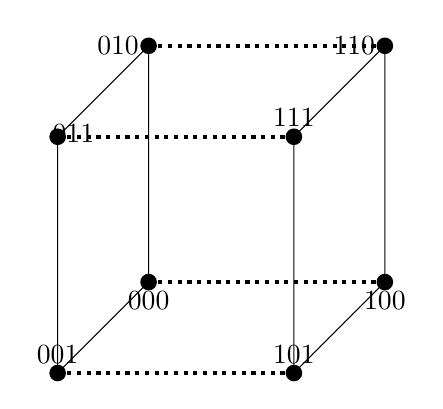
\begin{tikzpicture}[scale=1.5]
    % Define vertices and labels
    \coordinate[label=below:000] (000) at (0,0,0);
    \coordinate[label=above:001] (002) at (0,0,2);
    \coordinate[label=left:010] (020) at (0,2,0);
    \coordinate[label={[shift={(0.2,-0.2)}]above:011}] (022) at (0,2,2);
    \coordinate[label=below:100] (200) at (2,0,0);
    \coordinate[label=above:101] (202) at (2,0,2);
    \coordinate[label=left:110] (220) at (2,2,0);
    \coordinate[label=above:111] (222) at (2,2,2);

   \foreach \point in {(000),(002),(020),(022),(200),(202),(220),(222)} {
        \fill \point circle[radius=2pt];
    }
    % Draw edges
    \draw (000) -- (002) -- (022) -- (020) -- cycle;
    \draw (200) -- (202) -- (222) -- (220) -- cycle;
    \draw[dotted, line width=1.5pt]  (000) -- (200);
    \draw[dotted, line width=1.5pt] (002) -- (202);
    \draw[dotted, line width=1.5pt] (020) -- (220);
    \draw[dotted, line width=1.5pt] (022) -- (222);
\end{tikzpicture}
\]
    \item To connect corresponding vertices in these two \( Q_{n-1} \) graphs to form \( Q_n \), we need to add \( 2^{n-1} \) edges.
\end{enumerate}

Therefore, the total number of edges \( E_n \) in \( Q_n \) is:
\[ E_n = E_{n-1} + 2^{n-1} \]

This represents the recurrence relation for the number of edges in the \( Q_n \) cube graph in terms of \( E_{n-1} \). \\ \\


\section*{Answer 2}

To find the generating function for the sequence
\[ <1, 4, 7, 10, 13, \ldots >\]
We can use the formula for an arithmetic sequence.

The \( n^{th} \) term of an arithmetic sequence can be represented as:
\[ a_n = a_1 + (n - 1) \cdot d \]
where:
\begin{align*}
a_n & \text{ is the } n^{th} \text{ term of the sequence}, \\
a_1 & \text{ is the first term of the sequence}, \\
n & \text{ is the term number (position)}, \\
d & \text{ is the common difference between consecutive terms}.
\end{align*}
From the given sequence, we can observe that:
\[ a_1 = 1 \] (first term)
and
\[ d = 3 \] (since the difference between consecutive terms is 3).

Plugging these values into the formula, we get:
\[ a_n = 1 + (n - 1) \cdot 3 \]
which simplifies to:
\[ a_n = 1 + 3n - 3 \]
and further simplifies to:
\[ a_n = 3n - 2 \]

Starting with the basic generating functions:
\begin{enumerate}
    \item The generating function for the sequence \( <1, 1, 1, 1, \dots> \) is:
    \[ \frac{1}{1-x} \]

    \item Differentiating the above generating function gives:
    \[ \frac{d}{dx} \left( \frac{1}{1-x} \right) = \frac{1}{(1-x)^2} \]
    Which represents the sequence \( <1, 2, 3, 4, \dots> \).

    \item Using the scaling theorem:
    \begin{align*}
    &\text{Multiplying } \frac{1}{1-x} \text{ by 2 gives:} \\
    &\frac{2}{1-x} \\
    &\text{Which represents the sequence } <2, 2, 2, 2, \dots>.
    \end{align*}

    \begin{align*}
    &\text{Multiplying } \frac{1}{(1-x)^2} \text{ by 3 gives:} \\
    &\frac{3}{(1-x)^2} \\
    &\text{Which represents the sequence } <3, 6, 9, 12, \dots>.
    \end{align*}

    \item Subtracting the generating function for the sequence \( <2, 2, 2, 2, \dots> \) from the generating function for the sequence \( <3, 6, 9, 12, \dots> \) gives:
    \[ \frac{3}{(1-x)^2} - \frac{2}{1-x} \]
    This resulting generating function represents the sequence \( <1, 4, 7, 10, 13, \dots> \).
\end{enumerate}

Therefore, \( \frac{1+2x}{(1-x)^2} \)  is the generating function for the sequence \( <1, 4, 7, 10, 13, \dots> \).



\section*{Answer 3}

Define the generating function for the sequence \( a_n \) as:
\[ A(x) = \sum_{n=0}^{\infty} a_n x^n \]

Multiply both sides of the recurrence relation by \( x^n \) and sum over all valid values of \( n \):
\begin{align*}
\sum_{n=1}^{\infty} a_n x^n &= \sum_{n=1}^{\infty} a_{n-1} x^n + \sum_{n=1}^{\infty} 2^n x^n \\
\end{align*}

\begin{align*}
&= x\sum_{n=1}^{\infty} a_{n-1} x^{n-1} + \sum_{n=1}^{\infty} 2^n x^n
\end{align*}

We can write \( \sum_{n=1}^{\infty} a_{n-1} x^{n-1}\) as \( \sum_{n=0}^{\infty} a_{n} x^{n} = A(x) \) \\

Furthermore, we know that  \( \sum_{n=0}^{\infty} 2^n x^n = \frac{1}{1-2x} \),\\

Thus \( \sum_{n=1}^{\infty} 2^n x^n = \frac{1}{1-2x} - 1\)\\

Let's put them into the equation we have above:

\begin{align*}
A(x)-a_{0} &= xA(x) + \frac{1}{1-2x} - 1\\
A(x)-1 &= xA(x) + \frac{1}{1-2x} - 1\\
A(x)(1-x) &= \frac{1}{1-2x}\\
\end{align*}

Therefore, \( A(x) \) is:

\begin{align*}
A(x)&= \frac{1}{(1-2x)(1-x)} = \frac{B}{(1-x)} + \frac{C}{(1-2x)}  \ \ B,C \in \mathbb{R}\\
\end{align*}

So, we have \( B=-1\) and \(C=2\)

\begin{align*}
A(x)&= \frac{1}{(1-2x)(1-x)} = \frac{-1}{(1-x)} + \frac{2}{(1-2x)}  \\
\end{align*}

Since sequence of \( \frac{1}{1-x} \) generating function is \( <1, 1, 1, 1, \dots> \),\\

Sequence of \(\frac{-1}{(1-x)}\) is \( <-1, -1, -1, -1, \dots> \).\\

Since sequence of \( \frac{1}{1-2x} \) generating function is \( <1, 2, 4, 8, \dots> \),\\

Sequence of \(\frac{2}{(1-2x)}\) is \( <2, 4, 8, 16, \dots> \).\\

Therefore sequence of \( A(x) \) is \[ <1, 3, 7, 15, \dots, 2^{n+1}-1 , \dots>\].\\
Thus, we can say that: \[ a_n = 2^{n+1}-1\]



\section*{Answer 4}

\paragraph{a)}
\[
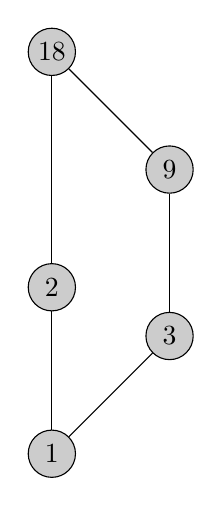
\begin{tikzpicture}[node distance=1.5cm]
  \tikzstyle{circ} = [circle, draw, fill=black!20, inner sep=0pt, minimum width=0.6cm]

  \node[circ] (18) {18};
  \node[circ, below right=of 18] (9) {9};
  \node[circ, below =of 9] (3) {3};
  \node[circ, below left=of 9] (2) {2};
  \node[circ, below left=of 3] (1) {1};

  \draw (18) -- (9);
  \draw (18) -- (2);
  \draw (9) -- (3);

  \draw (2) -- (1);
  \draw (3) -- (1);

\end{tikzpicture}
\]
\paragraph{b)}

\[
R = \begin{bmatrix}
1 & 1 & 1 & 1 & 1 \\
0 & 1 & 0 & 0 & 1 \\
0 & 0 & 1 & 1 & 1 \\
0 & 0 & 0 & 1 & 1 \\
0 & 0 & 0 & 0 & 1 \\
\end{bmatrix}
\]

\paragraph{c)}

To determine if \( (A, R) \) is a lattice, we need to check two conditions:

\begin{enumerate}
    \item Every pair of elements in \( A \) has both a least upper bound (LUB) and a greatest lower bound (GLB) in \( A \).
    \item The LUB and GLB are unique.
\end{enumerate}

Given the relation \( R \) defined as \( a \) divides \( b \), let's analyze the elements of \( A = \{1, 2, 3, 9, 18\} \):

\begin{enumerate}
    \item \textbf{Least Upper Bound (LUB) and Greatest Lower Bound (GLB) for each pair:}
    \begin{itemize}
        \item \( 1 \) and \( 2 \): LUB = \( 2 \), GLB = \( 1 \)
        \item \( 1 \) and \( 3 \): LUB = \( 3 \), GLB = \( 1 \)
        \item \( 1 \) and \( 9 \): LUB = \( 9 \), GLB = \( 1 \)
        \item \( 1 \) and \( 18 \): LUB = \( 18 \), GLB = \( 1 \)
        \item \( 2 \) and \( 3 \): LUB = \( 18 \) , GLB = \( 1 \)
        \item \( 2 \) and \( 9 \): LUB = \( 18 \), GLB = \( 1 \)
        \item \( 2 \) and \( 18 \): LUB = \( 18 \), GLB = \( 2 \)
        \item \( 3 \) and \( 9 \): LUB = \( 9 \), GLB = \( 3 \)
        \item \( 3 \) and \( 18 \): LUB = \( 18 \), GLB = \( 3 \)
        \item \( 9 \) and \( 18 \): LUB = \( 18 \), GLB = \( 9 \)
    \end{itemize}
    \item \textbf{Uniqueness of LUB and GLB:}
    \begin{itemize}
        \item For any pair, the LUB and GLB are unique based on the above analysis.
    \end{itemize}
\end{enumerate}

Given that every pair in \( A \) has both a LUB and a GLB, and these are unique for each pair, \( (A, R) \) satisfies the conditions of being a lattice.

Therefore, \( (A, R) \) is indeed a lattice.\\

\paragraph{d)}

The symmetric closure \( R^s \) of a relation \( R \) consists of all the ordered pairs \( (a, b) \) such that whenever \( (a, b) \) is in \( R \), then \( (b, a) \) is also in \( R^s \).

Given the relation \( R \) where \( a \) divides \( b \), we need to find the symmetric closure \( R^s \).

For each pair \( (a, b) \) in \( R \), we also need to include the pair \( (b, a) \) in \( R^s \).

From the previous matrix representation of \( R \):

\[
R = \begin{bmatrix}
1 & 1 & 1 & 1 & 1 \\
0 & 1 & 0 & 0 & 1 \\
0 & 0 & 1 & 1 & 1 \\
0 & 0 & 0 & 1 & 1 \\
0 & 0 & 0 & 0 & 1 \\
\end{bmatrix}
\]

For \( R^s \):

\begin{enumerate}
    \item \( (1, 2) \) is in \( R \), so we add \( (2, 1) \) to \( R^s \).
    \item \( (1, 3) \) is in \( R \), so we add \( (3, 1) \) to \( R^s \).
    \item \( (1, 9) \) is in \( R \), so we add \( (9, 1) \) to \( R^s \).
    \item \( (1, 18) \) is in \( R \), so we add \( (18, 1) \) to \( R^s \).
    \item \( (2, 18) \) is in \( R \), so we add \( (18, 2) \) to \( R^s \).
    \item \( (3, 9) \) is in \( R \), so we add \( (9, 3) \) to \( R^s \).
    \item \( (3, 18) \) is in \( R \), so we add \( (18, 3) \) to \( R^s \).
    \item \( (9, 18) \) is in \( R \), so we add \( (18, 9) \) to \( R^s \).
\end{enumerate}

But, since \( R \) only contains pairs where \( a \) divides \( b \) and does not contain pairs where \( b \) divides \( a \), the symmetric closure \( R^s \) will have all these pairs as well.

The matrix representation for \( R^s \) will therefore be:

\[
R = \begin{bmatrix}
1 & 1 & 1 & 1 & 1 \\
1 & 1 & 0 & 0 & 1 \\
1 & 0 & 1 & 1 & 1 \\
1 & 0 & 1 & 1 & 1 \\
1 & 1 & 1 & 1 & 1 \\
\end{bmatrix}
\]

This matrix captures the relation \( R^s \), which is the symmetric closure of \( R \).

\paragraph{e)}


In the relation \( R \) where \( a \) divides \( b \):

\begin{itemize}
    \item \( 2 \) does not divide \( 9 \). \\
    \( 9 \) does not divide \( 2 \). \\
    Since both \( (2,9) \) and \( (9,2) \) are not in the set of relation \( R \), we can say that \( 2 \) and \( 9 \) are not comparable in \( R \).
    \item \( 18 \) does not divide \( 3 \) but,\\
    \( 3 \) divides \( 18 \) since \( 3 \times 6 = 18 \)\\
    Thus, \( (3,18) \) is in the set of relation \( R \) . Therefore, \( 3 \) and \( 18 \) are comparable in \( R \).
\end{itemize}


\section*{Answer 5}


Let's solve each part step by step.

\subsection*{a) Reflexive and Symmetric Relations:}

For a relation to be reflexive on a set \( A \), it must contain the diagonal elements of the set, i.e., every element in \( A \) must be related to itself. Since a relation is reflexive if and only if it contains all the ordered pairs \( (a,a) \) where \( a \) is an element of \( A \), there are \( n \) such pairs.

For a relation to be symmetric on a set \( A \), if \( (a,b) \) is in the relation, then \( (b,a) \) must also be in the relation. However, this condition doesn't add any new ordered pairs, because if we have \( (a,a) \) for reflexivity, then by the definition of a relation being symmetric, \( (a,a) \) would also imply \( (a,a) \) again (since \( (a,a) \) implies \( (a,a) \) by reflexivity). Similarly, if we have some \( (a,b) \) with \( a \neq b \), then \( (b,a) \) would also be present in the relation by symmetry. However, by definition, we are already considering the relations that satisfy both reflexivity and symmetry.

Thus, for a given pair \( (a,b) \) in \( A \), we are essentially choosing between \( (a,b) \) and \( (b,a) \) or including both. This means there are \( 2^{\frac{n(n-1)}{2}} \) possible relations that are both reflexive and symmetric on \( A \).

Here's why:

For each distinct pair \( (a,b) \) in \( A \) (where \( a \neq b \)), we have two choices: to include \( (a,b) \) or to include \( (b,a) \). As there are \( \frac{n(n-1)}{2} \) such distinct pairs in \( A \), the total number of ways to choose relations that are both reflexive and symmetric is \( 2^{\frac{n(n-1)}{2}} \).

So, the number of different binary relations on \( A \) that are both reflexive and symmetric is \( 2^{\frac{n(n-1)}{2}} \).


\subsection*{b) Reflexive and Antisymmetric Relations:}

To determine the number of different binary relations on \( A \) that are both reflexive and antisymmetric, let's break it down step by step.

\begin{enumerate}
    \item \textbf{Reflexive Property}:
    For a relation to be reflexive on a set \( A \), it must contain the diagonal elements of the set, i.e., every element in \( A \) must be related to itself. Since a relation is reflexive if and only if it contains all the ordered pairs \( (a, a) \) where \( a \) is an element of \( A \), there are \( n \) such pairs.
    
    \item \textbf{Antisymmetric Property}:
    A relation \( R \) on a set \( A \) is antisymmetric if for all distinct elements \( a \) and \( b \) in \( A \), if \( (a, b) \) and \( (b, a) \) both belong to \( R \), then \( a = b \).
    
    Given the reflexive property, the diagonal elements are already covered. Now, consider any two distinct elements \( a \) and \( b \) in \( A \). There are three possibilities for their relation:
    
    \begin{enumerate}
        \item \( (a, b) \) belongs to the relation and \( (b, a) \) does not.
        \item \( (b, a) \) belongs to the relation and \( (a, b) \) does not.
        \item Neither \( (a, b) \) nor \( (b, a) \) belongs to the relation.
    \end{enumerate}
    
    For the relation to be antisymmetric, only one of the these possibilities can occur for any distinct pair \( (a, b) \). If both were present, the relation wouldn't be antisymmetric due to the given definition.
    
    Thus, for each distinct pair \( (a, b) \) in \( A \) (where \( a \neq b \)), there are 3 possibilities, and the number of such pairs is \( \frac{n(n-1)}{2} \). 
    
    So, for each of these \( \frac{n(n-1)}{2} \) pairs, there are 3 choices to make the relation antisymmetric.
\end{enumerate}

Therefore, the total number of different binary relations on \( A \) that are both reflexive and antisymmetric is \( 3^{\frac{n(n-1)}{2}} \).



\section*{Answer 6}

\begin{enumerate}
    \item \textbf{Antisymmetric Relation}:
An antisymmetric relation is one where for each directed edge in a graph, no edge exists that goes the other way. In other words, if an edge exists from element \( a \) to element \( b \), there cannot be an edge from \( b \) to \( a \). Mathematically, this means that if \( (a, b) \) is in the relation, then \( (b, a) \) cannot be in the relation unless \( a \) and \( b \) are the same element (i.e., \( a = b \)).
    \item \textbf{Transitive Closure}:
Now, let's consider the transitive closure of an antisymmetric relation. The transitive closure of a relation is the smallest transitive relation that contains the original relation as a subset. In other words, it ensures that if \( (a, b) \) and \( (b, c) \) are in the relation, then \( (a, c) \) must also be in the relation.
\end{enumerate}
Here's the interesting part: the transitive closure of an antisymmetric relation is not always antisymmetric! Let's see why:\\

Suppose we have an antisymmetric relation \( R \). \\
The transitive closure \( R^+ \) contains all pairs from \( R \) and additional pairs to satisfy the transitive property.\\
If \( (a, b) \) and \( (b, c) \) are in \( R^+ \), then by the transitive property, \( (a, c) \) must also be in \( R^+ \).\\
Since \( R \) is antisymmetric, if \( (a, b) \) is in \( R \), then \( (b, a) \) cannot be in \( R \). But if \( (a, b) \) and \( (b, c) \) are in \( R^+ \), but \( (a, c) \) may be in \( R^+ \), since there might be a path \(c\) to \(a\). Let's say \((c,d)\) and \( (d,a)\),therefore \( (c, a) \) can be in \( R^+ \). \\
Thus, \( R^+ \) does not satisfy the antisymmetric property. \\

Let's consider a counter example: \\

Consider a set, let's say \(A= \{1, 2, 3, 4\} \) \\

And relatin of \(A\) is \( R = \{(1, 3),(2, 1),(2, 3),(3, 4),(4, 1)\}\). \\


Let's find the transitive closure of these relations on \( \{1, 2, 3, 4\} \).

\begin{enumerate}
    \item \( R = \{(1, 2),(2, 1),(2, 3),(3, 4),(4, 1)\} \)

    Transitive Closure:
    \begin{align*}
    &M_R^* \\
    &= M_R \lor M_R^2  \lor M_R^3 \\
    &= \begin{bmatrix}
    0 & 0 & 1 & 0 \\
    1 & 0 & 1 & 0 \\
    0 & 0 & 0 & 1 \\
    1 & 0 & 0 & 0 \\
    \end{bmatrix} \lor \begin{bmatrix}
    0 & 0 & 0 & 1\\
    0 & 0 & 1 & 1 \\
    1 & 0 & 0 & 0 \\
    0 & 0 & 1 & 0 \\
    \end{bmatrix} \lor \begin{bmatrix}
    1 & 0 & 0 & 0 \\
    1 & 0 & 0 & 1 \\
    0 & 0 & 1 & 0 \\
    0 & 0 & 0 & 1 \\
    \end{bmatrix} \\
    &= \begin{bmatrix}
    1 & 0 & 1 & 1 \\
    1 & 0 & 1 & 1 \\
    1 & 0 & 1 & 1 \\
    1 & 0 & 1 & 1 \\
    \end{bmatrix}
    \end{align*}
\end{enumerate}

Note that \(\lor M_R^4\) is same with \(\lor M_R\) itself, therefore we do not need to write \(\lor M_R^4\) and keep writing the further \(M\)'s.\\

As you can see that \(M_R^*\) is not antisymmetric. Therefore we can say that transitive closure of an antisymmetric relation is not always antisymmetric.\\


\end{document}
